\begin{name}
	{\tenchude}
	{\tendethi}
	{\tentruong}
	{\thoigian}
\end{name}
\Opensolutionfile{ans}[ans/ans-De06HT]
% %%%=========Cau_1=========%%%
% \begin{ex}%[2D1Y2-2]
% 	\immini
% 	{
% 		Cho hàm số $y=f(x)$ có đồ thị như hình vẽ. Giá trị cực đại của hàm số bằng
% 		\choice
% 		{$0$}
% 		{\True $-1$}
% 		{$1$}
% 		{$-2$}
% 	}
% 	{
% 		\begin{tikzpicture}[smooth, line join=round, line cap = round, >=latex]
% 			\def\f(#1){(#1)^4-2*(#1)^2-1}
% 			\def\a{1}
% 			\pgfmathsetmacro\fa{\f(\a)}
% 			\draw[->] (-2.5,0) -- (2.5,0) node[below]{$x$};
% 			\draw[->] (0,-2.5) -- (0,1) node[right]{$y$};
% 			\clip (-2.5,-2.5) rectangle (2.5,1);
% 			\draw [smooth,domain=-1.7:1.7,samples=100] plot (\x,{\f(\x)});
% 			\draw[dashed] (-\a,0) node[above] {$\a$}--(-\a,\fa) -- (\a,\fa) -- (\a,0) node[above]{$\a$};
% 			\draw (0,0) node[below right] {$O$} (0,-\a-1) node[below left] {$-2$} (0,-\a) node[right] {$-\a$};
% 			\fill[black] (-1,0) circle (1pt);
% 			\fill[black] (1,0) circle (1pt);
% 		\end{tikzpicture}
% 	}
% 	\loigiai{
% 		Dựa vào đồ thị hàm số ta suy ra giá trị cực đại bằng $-1$.
% 	}
% \end{ex}
% %%%=========HetCau_1=========%%%

% %%%=========Cau_2=========%%%
% \begin{ex}%[2D3Y1-1]
% 	Cho hai hàm số $f(x),\,\,g(x)$ có đạo hàm liên tục trên $\mathbb{R}$. Xét các mệnh đề sau
% 	\begin{enumerate}[1)]
% 		\item $k\cdot\displaystyle\int f(x)\mathrm{d}x=\displaystyle\int k\cdot f(x)\mathrm{d}x$, với $ k $ là hằng số thực bất kì.
% 		\item $ \displaystyle\int\left[f(x)+g(x)\right]\mathrm{d}x=\displaystyle\int f(x)\mathrm{d}x+\displaystyle\int g(x)\mathrm{d}x$.
% 		\item $ \displaystyle\int\left[f(x)g(x)\right]\mathrm{d}x=\displaystyle\int f(x)\mathrm{d}x\cdot\displaystyle\int g(x)\mathrm{d}x. $ 
% 		\item $ \displaystyle\int f'(x)g(x)\mathrm{d}x+\displaystyle\int f(x)g'(x)\mathrm{d}x=f(x)g(x) $.
% 	\end{enumerate}
% 	Tổng số mệnh đề đúng là
% 	\choice
% 	{$2$}
% 	{\True $1$}
% 	{$4$}
% 	{$3$}
% 	\loigiai{
% 		Mệnh đề đúng là mệnh đề 2.
% 		Thật vậy ta có\\ $ \left(\displaystyle\int f(x)\mathrm{d}x+\displaystyle\int g(x)\mathrm{d}x\right)'=\left(\displaystyle\int f(x)\mathrm{d}x\right)'+\left(\displaystyle\int g(x)\mathrm{d}x\right)'=f(x)+g(x) $.\\
% 		Mệnh đề 1 sai. Nếu $ k=0 $ ta có $ VT=0 $; $ VP=\displaystyle\int 0\mathrm{d}x=C\ne VP $.\\
% 		Mệnh đề 3 sai. Phản ví dụ chọn $ f(x)=1 $; $ g(x)=0 $, suy ra $ VT=\displaystyle\int\left[f(x)g(x)\right]\mathrm{d}x=\displaystyle\int0\mathrm{d}x=C;\,VP=\displaystyle\int f(x)\mathrm{d}x.\displaystyle\int g(x)\mathrm{d}x=\displaystyle\int \mathrm{d}x\cdot\displaystyle\int0\mathrm{d}x=(x+C_1)\cdot C2 $.\\
% 		Mệnh đề 4 sai vì $VT=\displaystyle\int\left[f'(x)g(x)+f(x)g'(x)\right]\mathrm{d}x=\displaystyle\int\left[f(x)g(x)\right]'\mathrm{d}x=f(x)g(x)+C\ne VP $.
% 	}
% \end{ex}
% %%%=========HetCau_2=========%%%



% %%%=========Cau_3=========%%%
% \begin{ex}%[2D2Y1-2]
% 	Cho $ a $ là số thực dương tùy ý, $ \sqrt[4]{a^3} $ bằng
% 	\choice
% 	{\True $ a^{\tfrac{3}{4}} $}
% 	{$ a^{-\tfrac{3}{4}} $}
% 	{$ a^{\tfrac{4}{3}} $}
% 	{$ a^{-\tfrac{4}{3}} $}
% 	\loigiai{
% 		Ta có: $ \sqrt[4]{a^3}={a}^{\tfrac{3}{4}} $.
% 	}
% \end{ex}
% %%%=========HetCau_3=========%%%

% %%%=========Cau_4=========%%%
% \begin{ex}%[2H2Y1-1]
% 	Cho khối nón có chiều cao bằng $ 2a $ và bán kính đáy bằng $ a $. Thể tích của khối nón đã cho bằng
% 	\choice
% 	{$ 2\pi{a^3} $}
% 	{\True $ \dfrac{2\pi{a^3}}{3} $}
% 	{$ 4\pi{a^3} $}
% 	{$ \dfrac{4\pi{a^3}}{3} $}
% 	\loigiai{
% 		Thể tích của khối nón đã cho là: $ V=\dfrac{1}{3}\cdot h\cdot\pi {R}^2=\dfrac{1}{3}\cdot2a\cdot\pi\cdot a^2=\dfrac{2\pi a^3}{3}. $ 
% 	}
% \end{ex}
% %%%=========HetCau_4=========%%%

% %%%=========Cau_5=========%%%
% \begin{ex}%[2H3Y1-1]
% 	Trong không gian với hệ tọa độ $ Oxyz $, cho $ A\left(-1;2;-3\right) $ và $ B\left(-3;-1;1\right) $. Tọa độ của $ \overrightarrow{AB} $ là
% 	\choice
% 	{$ \overrightarrow{AB}=\left(-4;1;-2\right) $}
% 	{$ \overrightarrow{AB}=\left(2;3;-4\right) $}
% 	{\True $ \overrightarrow{AB}=\left(-2;-3;4\right) $}
% 	{$ \overrightarrow{AB}=\left(4;-3;4\right) $}
% 	\loigiai{
% 		Ta có $ \overrightarrow{AB}=(-3+1;-1-2;1+3)=(-2;-3;4) $.
% 	}
% \end{ex}
% %%%=========HetCau_5=========%%%

% %%%=========Cau_6=========%%%
% \begin{ex}%[2D1Y4-1]
% 	Cho hàm số $ y=\dfrac{x+1}{2x-2} $. Khẳng định nào sau đây đúng?
% 	\choice
% 	{Đồ thị hàm số có tiệm cận ngang là $ y=-\dfrac{1}{2} $}
% 	{Đồ thị hàm số có tiệm cận đứng là $ x=2 $}
% 	{\True Đồ thị hàm số có tiệm cận ngang là $ y=\dfrac{1}{2} $}
% 	{Đồ thị hàm số có tiệm cận đứng là $ x=\dfrac{1}{2} $}
% 	\loigiai{
% 		$ \lim\limits_{x\to +\infty}y=\dfrac{1}{2} $; $ \lim\limits_{x\to -\infty}y=\dfrac{1}{2} $ nên hàm số có tiệm cận ngang $ y=\dfrac{1}{2} $.\\
% 		$ \lim\limits_{x\to {1}^{+}}y=+\infty $; $ \lim\limits_{x\to {1}^{-}}y=-\infty $ nên hàm số có tiệm cận đứng $ x=1 $.
		
% 	}
% \end{ex}
% %%%=========HetCau_6=========%%%

% %%%=========Cau_7=========%%%
% \begin{ex}%[1D3Y3-1]
% 	Cho cấp số cộng $ \left(u_n\right) $ có số hạng đầu $ u_1=2 $ và công sai $ d=5 $. Giá trị của $ u_5 $ bằng
% 	\choice
% 	{$ 27 $}
% 	{$ 1250 $}
% 	{$ 12 $}
% 	{\True $ 22 $}
% 	\loigiai{
% 		Ta có $ u_5=u_1+4d=2+4\cdot5=22 $.
% 	}
% \end{ex}
% %%%=========HetCau_7=========%%%

% %%%=========Cau_8=========%%%
% \begin{ex}%[2D1Y5-1]
% 	\immini{
% 		Biết rằng đồ thị cho ở hình vẽ dưới đây là đồ thị của một trong 4 hàm số cho trong 4 phương án $ A,\,B,\,C,\,D $. Đó là đồ thị hàm số nào?
% 		\choice
% 		{$ y=x^3-5x^2+4x+3 $}
% 		{$ y=2x^3-6x^2+4x+3 $}
% 		{\True $ y=x^3-4x^2+3x+3 $}
% 		{$ y=2x^3+9x^2-11x+3 $}
% 	}
% 	{
% 		\begin{tikzpicture}[smooth,line join = round, line cap = round, >= stealth,scale=0.7]
% 			\draw[->] (-1.5,0) -- (3.5,0) node[below] {\footnotesize $ x $};
% 			\draw[->] (0,-1) -- (0,4.3) node[right] {\footnotesize $ y $};
% 			\draw[smooth,samples=100,domain=-0.6:3.2] plot(\x,{(\x)^3-4*(\x)^2+3*(\x)+3});
% 			\draw[dashed] (0,3) node[left] {\footnotesize $ 3 $} -- (1,3) -- (1,0) node[below] {\footnotesize $ 1 $};
% 			\draw[dashed] (0,1) node[above right] {\footnotesize $ 1 $} -- (2,1) -- (2,0) node[below] {\footnotesize $ 2 $};
% 			\fill[black] (1,0) circle (1pt);
% 			\fill[black] (2,0) circle (1pt);
% 			\fill[black] (0,1) circle (1pt);
% 			\fill[black] (0,3) circle (1pt);
% 		\end{tikzpicture}
% 	}
% 	\loigiai{
% 		Đồ thị đã cho đi qua các điểm $ M(1;3) $, $ N(2;1) $ và $ P(0;3) $.\\
% 		Xét phương án A ta có điểm $ N(2;1) $ không thuộc vào đồ thị hàm số $ y=x^3-5x^2+4x+3 $.\\
% 		Xét phương án B ta có điểm $ N(2;1) $ không thuộc vào đồ thị hàm số $ y=2x^3-6x^2+4x+3 $.\\
% 		Xét phương án D ta có điểm $ N(2;1) $ không thuộc vào đồ thị hàm số $ y=2x^3+9x^2-11x+3 $.\\
% 		Xét phương án C ta có cả ba điểm $ M(1;3) $, $ N(2;1) $ và $ P(0;3) $ đều thuộc vào đồ thị hàm số \linebreak $ y=x^3-4x^2+3x+3 $.
% 	}
% \end{ex}
% %%%=========HetCau_8=========%%%

% %%%=========Cau_9=========%%%
% \begin{ex}%[2H3Y2-4]
% 	Trong không gian $ Oxyz $, mặt phẳng $ (P)\colon x+2y-6z-1=0 $ đi qua điểm nào dưới đây?
% 	\choice
% 	{\True $ B\left(-3;2;0\right) $}
% 	{$ D\left(1;2;-6\right) $}
% 	{$ A\left(-1;-4;1\right) $}
% 	{$ C\left(-1;-2;1\right) $}
% 	\loigiai{
% 		Thay tọa độ điểm $ B $ ta có $ \colon-3+2\cdot2-6\cdot0-1=0 $. 
% 	}
% \end{ex}
% %%%=========HetCau_9=========%%%

% %%%=========Cau_10=========%%%
% \begin{ex}%[2H3Y3-1]
% 	Trong không gian $ Oxyz $ cho đường thẳng $ d\colon\dfrac{x-3}{1}=\dfrac{y+1}{-2}=\dfrac{z-5}{3} $. Vectơ nào sau đây là một vectơ chỉ phương của đường thẳng $ d $?
% 	\choice
% 	{\True $ \vec{u}_2=(1;-2;3) $}
% 	{$ \vec{u}_3=(2;6;-4) $}
% 	{$ \vec{u}_4=(-2;-4;6) $}
% 	{$ \vec{u}_1=(3;-1;5) $}
% 	\loigiai{
% 		Ta thấy đường thẳng d có một vectơ chỉ phương có tọa độ $ \vec{u}_2=(1;-2;3) $.
% 	}
% \end{ex}
% %%%=========HetCau_10=========%%%

% %%%=========Cau_11=========%%%
% \begin{ex}%[2D3Y1-1]
% 	Hàm số nào sau đây là một nguyên hàm của hàm số $ f(x)=3^{2x} $?
% 	\choice
% 	{$ F(x)=2\cdot3^{2x}\cdot\ln 3 $}
% 	{\True $ F(x)=\dfrac{3^{2x}}{2\cdot\ln 3}+2 $}
% 	{$ F(x)=\dfrac{3^{2x}}{3\cdot\ln 2} $}
% 	{$ F(x)=\dfrac{3^{2x}}{3\cdot\ln 3}-1 $}
% 	\loigiai{
% 		Ta có: $ \displaystyle\int{3}^{2x}\mathrm{d}x=\dfrac{1}{2}\displaystyle\int{3}^{2x}\cdot2\mathrm{d}x=\dfrac{1}{2}\displaystyle\int{3}^{2x}\mathrm{d}(2x)=\dfrac{1}{2}\cdot \dfrac{3^{2x}}{\ln 3}+C $.\\
% 		Cho hằng số $ C=2 $ ta được đáp án.
% 	}
% \end{ex}
% %%%=========HetCau_11=========%%%

% %%%=========Cau_12=========%%%
% \begin{ex}%[2D4Y2-1]
% 	Cho số phức $ z_1=2+3i $, $ z_2=-4-5i $. Tính $ z=z_1+z_2 $.
% 	\choice
% 	{$ z=-2+2i $}
% 	{$ z=2-2i $}
% 	{\True $ z=-2-2i $}
% 	{$ z=2+2i $}
% 	\loigiai{
% 		Ta có: $ z_1+z_2=(2+3i)+(-4-5i)=2-4+3i-5i=-2-2i $.\\
% 		Vậy $ z=-2-2i $.
% 	}
% \end{ex}
% %%%=========HetCau_12=========%%%

% %%%=========Cau_13=========%%%
% \begin{ex}%[2D4Y1-2]
% 	Trong mặt phẳng $ Oxy $, điểm nào sau đây biểu diễn số phức $ z=2+i $?
% 	\choice
% 	{$ P(2;-1) $}
% 	{$ Q(1;2) $}
% 	{$ M(2;0) $}
% 	{\True $ N(2;1) $}
% 	\loigiai{
% 		Số phức $ z=a+bi $ có điểm biểu diễn $ (a;b) $ nên số phức $ z=2+i $ có điểm biểu diễn là $ N(2;1) $.
% 	}
% \end{ex}
% %%%=========HetCau_13=========%%%

% %%%=========Cau_14=========%%%
% \begin{ex}%[2D2Y5-1]
% 	Nghiệm của phương trình $ 2^{1-x}=4 $ là
% 	\choice
% 	{$ x=3 $}
% 	{$ x=-3 $}
% 	{\True $ x=-1 $}
% 	{$ x=1 $}
% 	\loigiai{
% 		Ta có $ 2^{1-x}=4\Leftrightarrow 2^{1-x}=2^2\Leftrightarrow 1-x=2\Leftrightarrow x=-1 $.
% 	}
% \end{ex}
% %%%=========HetCau_14=========%%%

% %%%=========Cau_15=========%%%
% \begin{ex}%[2H3Y1-3]
% 	Trong không gian với hệ tọa độ $ Oxyz $, cho mặt cầu $ (S)\colon\left(x-3\right)^2+\left(y+1\right)^2+\left(z+2\right)^2=8 $. Khi đó tâm $ I $ và bán kính $ R $ của mặt cầu là
% 	\choice
% 	{$ I\left(3;-1;-2\right),\,R=4 $}
% 	{\True $ I\left(3;-1;-2\right),\,R=2\sqrt{2} $}
% 	{$ I\left(-3;1;2\right),\,R=2\sqrt{2} $}
% 	{$ I\left(-3;1;2\right),\,R=4 $}
% 	\loigiai{
% 		Mặt cầu $ (S) $ có tâm $ I(3;-1;-2) $ và bán kính $ R=2\sqrt{2} $.
% 	}
% \end{ex}
% %%%=========HetCau_15=========%%%

% %%%=========Cau_16=========%%%
% \begin{ex}%[2H2B1-3]
% 	Quay hình vuông $ ABCD $ cạnh $ a $ xung quanh một cạnh. Thể tích của khối trụ được tạo thành là
% 	\choice
% 	{$ 3\pi a^3 $}
% 	{$ \dfrac{1}{3}\pi a^3 $}
% 	{$ 2\pi a^3 $}
% 	{\True $ \pi a^3 $}
% 	\loigiai{
% 		Quay hình vuông ABCD cạnh $ a $ xung quanh một cạnh ta được khối trụ có chiều cao bằng $ a $ và diện tích đáy là $ \pi a^2 $.\\
% 		Vậy thể tích của khối trụ là $ \pi a^3 $.
% 	}
% \end{ex}
% %%%=========HetCau_16=========%%%

% %%%=========Cau_17=========%%%
% \begin{ex}%[2D1Y1-2]
% 	Hàm số $ y=f(x) $ có bảng biến thiên dưới đây nghịch biến trên khoảng nào?
% 	\begin{center}
% 		\begin{tikzpicture}
% 			\tkzTabInit[nocadre,lgt=1,espcl=2.5,deltacl=0.7] {$ x $ /0.7, $ y' $ /0.7, $ y $ /2.5} {$ -\infty $, $ -3 $, $ 0 $, $ 3 $, $ +\infty $}
% 			\tkzTabLine {,-,0,+,0,-,0,+,}
% 			\tkzTabVar {+/ $ +\infty $,-/ $ -2 $,+/ $ 1 $,-/ $ -3 $,+/ $ +\infty $}
% 		\end{tikzpicture}
% 	\end{center}
% 	\choice
% 	{\True $ \left(0;3\right) $}
% 	{$ \left(3;+\infty\right) $}
% 	{$ \left(-3;3\right) $}
% 	{$ \left(-\infty;-2\right) $}
% 	\loigiai{
% 		Dựa vào bảng biến thiên của hàm số ta thấy hàm số trên nghịch biến trên các khoảng $ (-\infty;-3) $ và $ (0;3) $.
% 	}
% \end{ex}
% %%%=========HetCau_17=========%%%

% %%%=========Cau_18=========%%%
% \begin{ex}%[2H1B3-2]
% 	Thể tích $ V $ của khối lăng trụ tam giác đều có tất cả các cạnh bằng $ a $ là
% 	\choice
% 	{$ V=\dfrac{a^3\sqrt{2}}{3} $}
% 	{\True $ V=\dfrac{a^3\sqrt{3}}{4} $}
% 	{$ V=\dfrac{a^3\sqrt{3}}{2} $}
% 	{$ V=\dfrac{a^3\sqrt{2}}{4} $}
% 	\loigiai{
% 		Ta có $ S_{ABC}=\dfrac{a^2\sqrt{3}}{4} $. Vậy $ V=a\cdot\dfrac{a^2\sqrt{3}}{4}=\dfrac{a^3\sqrt{3}}{4} $.
% 	}
% \end{ex}
% %%%=========HetCau_18=========%%%

% %%%=========Cau_19=========%%%
% \begin{ex}%[1D2Y2-1]
% 	Cho tập $ A $ có $ 26 $ phần tử. Hỏi $ A $ có bao nhiêu tập con gồm $6$ phần tử?
% 	\choice
% 	{$ \mathrm{A}_{26}^6 $}
% 	{$ 26 $}
% 	{$ \mathrm{A}_6 $}
% 	{\True $ \mathrm{C}_{26}^6 $}
% 	\loigiai{
% 		Số tập con gồm $6$ phần tử của $ A $ bằng số tổ hợp chập $ 6 $ của $ 26 $ phần tử. Vậy số tập con là $ \mathrm{C}_{26}^6 $.
% 	}
% \end{ex}
% %%%=========HetCau_19=========%%%

% %%%=========Cau_20=========%%%
% \begin{ex}%[2D2B4-2]
% 	Hàm số $ f(x)=\mathrm{e}^{\sqrt{x^2+1}} $ có đạo hàm là
% 	\choice
% 	{$ f'(x)=\dfrac{2x}{\sqrt{x^2+1}}\cdot\mathrm{e}^{\sqrt{x^2+1}} $}
% 	{$ f'(x)=\dfrac{x}{\sqrt{x^2+1}}\cdot\mathrm{e}^{\sqrt{x^2+1}}\cdot\ln 2 $}
% 	{$ f'(x)=\dfrac{x}{2\sqrt{x^2+1}}\cdot\mathrm{e}^{\sqrt{x^2+1}} $}
% 	{\True $ f'(x)=\dfrac{x}{\sqrt{x^2+1}}\cdot\mathrm{e}^{\sqrt{x^2+1}} $}
% 	\loigiai{
% 		$ f'(x)=\left(\sqrt{x^2+1}\right)'\cdot\mathrm{e}^{\sqrt{x^2+1}}=\dfrac{2x}{2\sqrt{x^2+1}}\cdot\mathrm{e}^{\sqrt{x^2+1}}=\dfrac{x}{\sqrt{x^2+1}}\cdot\mathrm{e}^{\sqrt{x^2+1}} $.
% 	}
% \end{ex}
% %%%=========HetCau_20=========%%%

% %%%=========Cau_21=========%%%
% \begin{ex}%[2D4K3-3]
% 	Cho số phức $z$ có phần thực là số nguyên và thỏa mãn $ | z|-2\overline{z}=-7+3i+z $. Tính mô-đun của số phức $ w=1-z+z^2 $. 
% 	\choice
% 	{$ | w|=\sqrt{445} $}
% 	{$ | w|=\sqrt{37} $}
% 	{\True $ | w|=\sqrt{457} $}
% 	{$ | w|=\sqrt{425} $}
% 	\loigiai{
% 		Gọi $ z=a+bi $; $ a,b\in \mathbb{R};\,i^2=-1 $; $ a $ là số nguyên. Theo đề ta có
% 		$$\begin{aligned}
% 			|z|-2\overline{z}=-7+3i+z&\Leftrightarrow \sqrt{a^2+b^2}-2a+2bi=-7+3i+a+bi\\
% 			&\Leftrightarrow (\sqrt{a^2+b^2}-2a)+2bi=(-7+a)+(3+b)i\\
% 			&\Leftrightarrow\begin{cases}
% 				\sqrt{a^2+b^2}-2a=-7+a \\ 
% 				2b=3+b
% 			\end{cases}\Leftrightarrow\begin{cases}
% 				\sqrt{a^2+9}=3a-7 \\ 
% 				b=3
% 			\end{cases}\\
% 			&\Leftrightarrow\begin{cases}
% 				a\ge \dfrac{7}{3}\\ 
% 				8a^2-42a+40=0 \\ 
% 				b=3
% 			\end{cases}\Leftrightarrow\begin{cases}
% 				a\ge \dfrac{7}{3}\\ 
% 				\left[\begin{aligned}
% 					& a=4 \\ 
% 					& a=\dfrac{5}{4}
% 				\end{aligned}\right.\\ 
% 				b=3
% 			\end{cases}\Leftrightarrow\begin{cases}
% 				a=4 \\ 
% 				b=3
% 			\end{cases}
% 		\end{aligned}$$
% 		Khi đó $ z=4+3i $.
% 		Vậy $ w=1-z+z^2=4+21i\Rightarrow \bigg| w \bigg|=\sqrt{457} $.
% 	}
% \end{ex}
% %%%=========HetCau_21=========%%%

% %%%=========Cau_22=========%%%
% \begin{ex}%[2D2Y6-2]
% 	Tìm tập nghiệm $ S $ của bất phương trình $ \left(\dfrac{1}{2}\right)^x>8 $. 
% 	\choice
% 	{\True $ S=(-\infty;-3) $}
% 	{$ S=(3;+\infty) $}
% 	{$ S=(-3;+\infty) $}
% 	{$ S=(-\infty;3) $}
% 	\loigiai{
% 		Ta có: $ \left(\dfrac{1}{2}\right)^x>8\Leftrightarrow {2}^{-x}>2^3\Leftrightarrow -x>3\Leftrightarrow x<-3 $.\\
% 		Vậy bất phương trình có tập nghiệm là $ S=(-3;+\infty) $.
% 	}
% \end{ex}
% %%%=========HetCau_22=========%%%

% %%%=========Cau_23=========%%%
% \begin{ex}%[2H1B3-2]
% 	Cho khối chóp $ S.ABC $ có đáy $ ABC $ là tam giác vuông tại $ A $, biết $ AB=a $, $ AC=2a $. Mặt bên $ SAB $ là tam giác đều và nằm trong mặt phẳng vuông góc với mặt phẳng đáy. Tính theo $ a $ thể tích khối chóp $ S.ABC $. 
% 	\choice
% 	{$ \dfrac{a^3\sqrt{3}}{2} $}
% 	{$ \dfrac{a^3\sqrt{3}}{3} $}
% 	{\True $ \dfrac{a^3\sqrt{3}}{6} $}
% 	{$ \dfrac{a^3\sqrt{3}}{4} $}
% 	\loigiai{
% 		\immini{
% 			$ \triangle ABC $ vuông tại $ A $ nên
% 			$ S_{\triangle ABC}=\dfrac{1}{2}AB\cdot AC=\dfrac{1}{2}\cdot a\cdot2a=a^2 $.\\
% 			Gọi $ H $ là trung điểm $ AB $ $ \Rightarrow SH=\dfrac{a\sqrt{3}}{2} $.\\
% 			$ \triangle SAB $ đều $ \Rightarrow SH\perp AB $ 
% 			$ \Rightarrow SH\perp (ABC) $ (vì $ (SAB)\perp (ABC) $).\\
% 			$ \Rightarrow {V_{S.ABC}}=\dfrac{1}{3}SH\cdot{S}_{\triangle ABC}=\dfrac{a^3\sqrt{3}}{6} $.
% 		}
% 		{
% 			\begin{tikzpicture}[smooth, line join=round, line cap=round, font=\scriptsize,scale=0.8]
% 				\path
% 				(0,0) coordinate (A)
% 				($ (A)+(0:5) $) coordinate (C)
% 				($ (A)+(-45:2.5) $) coordinate (B)
% 				($ (A)!0.5!(B) $) coordinate (H)
% 				($ (H)+(90:3) $) coordinate (S);
% 				\draw (S)--(A)--(B)--(S)--(C)--(B) (S)--(H);
% 				\draw[dashed] (A)--(C);
% 				\foreach \x/\g in {A/180,S/90,C/0,H/180,B/-90}
% 				\fill [black] (\x) circle (1pt) + (\g:3mm) node {$ \x $};
% 				\draw pic[draw,angle radius=2mm] {right angle = S--H--A};
% 			\end{tikzpicture}
% 		}
% 	}
% \end{ex}
% %%%=========HetCau_23=========%%%

% %%%=========Cau_24=========%%%
% \begin{ex}%[2D1B3-2]
% 	Giá trị nhỏ nhất của hàm số $ y=\sqrt{x-1}+\sqrt{2-x}+2019 $ bằng
% 	\choice
% 	{$ 2025 $}
% 	{\True $ 2020 $}
% 	{$ 2023 $}
% 	{$ 2021 $}
% 	\loigiai{
% 		Tập xác định của hàm số là $ \mathscr{D}=[1;2] $, hàm số $ y=\sqrt{x-1}+\sqrt{2-x}+2019 $ liên tục trên đoạn $ [1;2] $.\\
% 		Ta có $ y'=\dfrac{1}{2\sqrt{x-1}}-\dfrac{1}{2\sqrt{2-x}}=0\Leftrightarrow \begin{cases}\sqrt{x-1}=\sqrt{2-x}\\ x\ne 1,\,x\ne 2
% 		\end{cases}\Leftrightarrow\begin{cases}x-1=2-x \\ x\ne 1,\,x\ne 2
% 		\end{cases}\Leftrightarrow x=\dfrac{3}{2} $.\\
% 		$ y(1)=2020 $; $ y(2)=2020 $; $ y\left(\dfrac{3}{2}\right)=2019+\sqrt{2} $.\\
% 		Vậy giá trị nhỏ nhất của hàm số $ y=\sqrt{x-1}+\sqrt{2-x}+2019 $ là $ 2020 $.
% 	}
% \end{ex}
% %%%=========HetCau_24=========%%%

% %%%=========Cau_25=========%%%
% \begin{ex}%[2D2B4-3]
% 	Trong các hàm số sau, hàm số nào luôn đồng biến trên khoảng $ \left(-\infty;+\infty\right) $?
% 	\choice
% 	{$ y=\sin x $}
% 	{$ y=x^4+1 $}
% 	{$ y=\ln x $}
% 	{\True $ y=x^5+5x $}
% 	\loigiai{
% 		Ta có $ y'=5x^4+5>0,\forall x\in (-\infty;+\infty) $.
% 		Do đó hàm số $ y=x^5+5x $ luôn đồng biến trên khoảng $ (-\infty;+\infty) $.
% 	}
% \end{ex}
% %%%=========HetCau_25=========%%%

% %%%=========Cau_26=========%%%
% \begin{ex}%[1H3B5-3]
% 	Cho hình chóp $ S.ABC $ có đáy $ ABC $ là tam giác vuông tại $ A $, $ AB=a $, $ AC=a\sqrt{3} $. Tam giác $ SBC $ đều và nằm trong mặt phẳng vuông với đáy. Tính khoảng cách $ d $ từ $ B $ đến mặt phẳng $ \left(SAC\right) $.
% 	\choice
% 	{$ d=a $}
% 	{\True $ d=\dfrac{2a\sqrt{39}}{13} $}
% 	{$ d=\dfrac{a\sqrt{3}}{2} $}
% 	{$ d=\dfrac{a\sqrt{39}}{13} $}
% 	\loigiai{
% 		\immini{
% 			Gọi $ H $ là trung điểm của $ BC $, suy ra $ SH\perp BC\Rightarrow SH\perp (ABC) $.\\
% 			Gọi $ K $ là trung điểm $ AC $, suy ra $ HK\perp AC $.\\
% 			Kẻ $ HE\perp SK $ $ (E\in SK) $.\\
% 			Khi đó $ \mathrm{d}\left(B,(SAC)\right) =2\mathrm{d}\left(H,(SAC)\right) $ $ =2HE=2\cdot\dfrac{SH\cdot HK}{\sqrt{SH^2+HK^2}}=\dfrac{2a\sqrt{39}}{13} $.
% 		}
% 		{
% 			\begin{tikzpicture}[smooth,line join=round,line cap=round,font=\scriptsize,scale=0.8]
% 				\path 
% 				(0,0) coordinate (B)
% 				($ (B)+(-30:3) $) coordinate (C)
% 				($ (B)+(0:4) $) coordinate (A)
% 				($ (B)!0.5!(C) $) coordinate (H)
% 				($ (H)+(90:3) $) coordinate (S)
% 				($ (A)!0.5!(C) $) coordinate (K)
% 				($ (S)!0.5!(K) $) coordinate (E);
% 				\draw (S)--(B)--(C)--(A)--cycle (H)--(S)--(K) (S)--(C);
% 				\draw[dashed] (B)--(A)--(H)--(K) (H)--(E);
% 				\draw pic[draw, angle radius=1.5mm] {right angle = S--H--B};
% 				\draw pic[draw, angle radius=1.5mm] {right angle = S--E--H};
% 				\draw pic[draw, angle radius=1.5mm] {right angle = H--K--C};
% 				\draw pic[draw, angle radius=1.5mm] {right angle = B--A--C};
% 				\foreach \x/\g in {S/90,B/180,H/-135,C/-90,K/0,A/0,E/0}
% 				\fill [black] (\x) circle (1pt)+ (\g:3mm) node {$ \x $};
% 			\end{tikzpicture}
% 		}
% 	}
% \end{ex}
% %%%=========HetCau_26=========%%%

% %%%=========Cau_27=========%%%
% \begin{ex}%[1D2B5-3]
% 	Có $ 13 $ học sinh của một trường THPT đạt danh hiệu học sinh xuất sắc trong đó khối $ 12 $ có $ 8 $ học sinh nam và $ 3 $ học sinh nữ, khối $ 11 $ có $ 2 $ học sinh nam. Chọn ngẫu nhiên $ 3 $ học sinh bất kỳ để trao thưởng, tính xác suất để $ 3 $ học sinh được chọn có cả nam và nữ đồng thời có cả khối $ 11 $ và khối $ 12 $.
% 	\choice
% 	{$ \dfrac{229}{286} $}
% 	{$ \dfrac{24}{143} $}
% 	{$ \dfrac{27}{143} $}
% 	{\True $ \dfrac{57}{286} $}
% 	\loigiai{
% 		Không gian mẫu là số cách chọn ngẫu nhiên 3 học sinh từ 13 học sinh.\\
% 		Suy ra số phần tử của không gian mẫu là $ \big| \Omega \big|=\mathrm{C}_{13}^3=286 $.\\
% 		Gọi $ A $ là biến cố " $ 3 $ học sinh được chọn có cả nam và nữ đồng thời có cả khối $ 11 $ và khối $ 12 $ ". Ta có các trường hợp thuận lợi cho biến cố $ A $ là
% 		\begin{enumerate}[$ \bullet $]
% 			\item TH1: Chọn $ 1 $ học sinh khối $ 11 $; $ 1 $ học sinh nam khối $ 12 $ và $ 1 $ học sinh nữ khối 12 nên có $ \mathrm{C}_2^1\cdot \mathrm{C}_8^1\cdot \mathrm{C}_3^1=48 $ cách.
% 			\item TH2: Chọn $ 1 $ học sinh khối $ 11 $; $ 2 $ học sinh nữ khối $ 12 $ có $ \mathrm{C}_2^1\cdot \mathrm{C}_3^2=6 $ cách.
% 			\item TH3: Chọn 2 học sinh khối $ 11 $; $ 1 $ học sinh nữ khối $ 12 $ có $ \mathrm{C}_2^2 \cdot \mathrm{C}_3^1=3 $ cách.
% 		\end{enumerate}
% 		Suy ra số phần tử của biến cố $ A $ là $ \big| {\Omega}_A \big|=48+6+3=57 $.\\
% 		Vậy xác suất cần tính $ P(A)=\dfrac{\big| {\Omega}_A \big|}{\big| \Omega \big|}=\dfrac{57}{286} $. 
% 	}
% \end{ex}
% %%%=========HetCau_27=========%%%

% %%%=========Cau_28=========%%%
% \begin{ex}%[2D3B1-2]
% 	Hàm số nào trong các hàm số sau đây có một nguyên hàm bằng $ y=\cos^2x $?
% 	\choice
% 	{$ y=\dfrac{-\cos^3x}{3}+C\,\left(C\in\mathbb{R}\right) $}
% 	{\True $ y=-\sin 2x $}
% 	{$ y=\sin 2x+C\,\left(C\in\mathbb{R}\right) $}
% 	{$ y=\dfrac{\cos^3x}{3} $}
% 	\loigiai{
% 		Ta có $ \left(\cos^2x\right)'=2\cos x\cdot(-\sin x)=-\sin 2x $.\\
% 		Vậy hàm số $ y=-\sin 2x $ có một nguyên hàm là $ y=\cos^2x $.
		
% 	}
% \end{ex}
% %%%=========HetCau_28=========%%%

% %%%=========Cau_29=========%%%
% \begin{ex}%[1H3K4-2]
% 	Cho hình chóp tứ giác đều có tất cả các cạnh đều bằng $ a $. Tính cosin của góc giữa một mặt bên và mặt đáy.
% 	\choice
% 	{$ \dfrac{1}{3} $}
% 	{$ \dfrac{\sqrt{2}}{2} $}
% 	{$ \dfrac{1}{2} $}
% 	{\True $ \dfrac{\sqrt{3}}{3} $}
% 	\loigiai{
% 		\immini{
% 			Gọi tứ diện đều là $ S. ABCD $, gọi $ O=AC\cap BD\Rightarrow SO\perp (ABCD) $.\\
% 			Gọi là $ I $ trung điểm của $ BC $.\\
% 			Khi đó ta có $ \begin{cases}
% 				BC\perp SO \\ 
% 				BC\perp OI
% 			\end{cases}\Rightarrow BC\perp (SOI)\Rightarrow BC\perp SI $.\\
% 			Do đó $\left((SBC),(ABCD)\right)=\left(\widehat{SI,OI}\right)=\widehat{SIO} $.\\
% 			Ta có $ OI=\dfrac{a}{2},\,SI=\sqrt{SB^2}-BI^2=\sqrt{a^2-\left(\dfrac{a}{2}\right)^2}=\dfrac{a\sqrt{3}}{2} $.\\
% 			Tam giác $ SOI $ vuông tại $ O $ $ \Rightarrow \cos \widehat{SIO}=\dfrac{OI}{SI}=\dfrac{\dfrac{a}{2}}{\dfrac{a\sqrt{3}}{2}}=\dfrac{\sqrt{3}}{3} $.
% 		}
% 		{
% 			\begin{tikzpicture}[smooth,line join=round,line cap=round,scale=0.7]
% 				\path 
% 				(0,0) coordinate (A)
% 				($ (A)+(-135:3) $) coordinate (D)
% 				($ (A)+(0:5) $) coordinate (B)
% 				($ (B)+(D)-(A) $) coordinate (C)
% 				($ (A)!0.5!(C) $) coordinate (O)
% 				($ (O)+(90:5) $) coordinate (S)
% 				($ (C)!0.5!(B) $) coordinate (I);
% 				\draw [dashed] (S)--(A)--(D)--(B)--(A)--(C) (S)--(O)--(I);
% 				\draw (S)--(D)--(C)--(S)--(B)--(C) (S)--(I);
% 				\begin{scope}
% 					\clip (S)--(I)--(O);
% 					\draw[fill=cyan!60,opacity=0.7] (I) circle(3mm);
% 				\end{scope}
% 				\foreach \x/\g in {A/180,D/180,C/0,B/0,I/0,O/-90,S/90}
% 				\fill[black] (\x) circle (1pt) + (\g:3mm) node {$ \x $};
% 			\end{tikzpicture}
% 		}
% 	}
% \end{ex}
% %%%=========HetCau_29=========%%%

% %%%=========Cau_30=========%%%
% \begin{ex}%[2D2K5-2]
% 	Tổng các lập phương các nghiệm của phương trình $ \log_2x\cdot\log_3\left(2x-1\right)=2\log_2x $ bằng
% 	\choice
% 	{$ 26 $}
% 	{\True $ 216 $}
% 	{$ 126 $}
% 	{$ 6 $}
% 	\loigiai{
% 		Điều kiện:
% 		$ \begin{cases}
% 			x>0 \\ 
% 			2x-1>0
% 		\end{cases}\Leftrightarrow x>\dfrac{1}{2} $.\\
% 		Phương trình đã cho tương đương
% 		\begin{center}
% 			$ \begin{aligned}[t]
% 				& \log_2x\cdot\log_3(2x-1)-2\log_2x=0 
% 				\Leftrightarrow	\log_2x\left[\log_3(2x-1)-2\right]=0\\
% 				\Leftrightarrow &\left[\begin{aligned}
% 					& {\log}_2x=0 \\ 
% 					& {\log}_3(2x-1)-2=0
% 				\end{aligned}\right. \Leftrightarrow \left[\begin{aligned}
% 					& x=1\\
% 					& 2x-1=9
% 				\end{aligned}\right.\Leftrightarrow \left[\begin{aligned}
% 					& x=1\\
% 					& x=5.
% 				\end{aligned}\right.
% 			\end{aligned} $ \\
% 		\end{center}
% 		Tổng lập phương các nghiệm là: $ 1^3+5^3=126 $.
% 	}
% \end{ex}
% %%%=========HetCau_30=========%%%

% %%%=========Cau_31=========%%%
% \begin{ex}%[2H3B1-3]
% 	Trong không gian $ Oxyz $, cho hai điểm $ A\left(4;-1;3\right) $, $ B\left(0;1;-5\right) $. Phương trình mặt cầu đường kính $ AB $ là
% 	\choice
% 	{\True $ \left(x-2\right)^2+y^2+\left(z+1\right)^2=21 $}
% 	{$ \left(x-2\right)^2+y^2+\left(z-1\right)^2=17 $}
% 	{$ \left(x-1\right)^2+\left(y-2\right)^2+z^2=27 $}
% 	{$ \left(x+2\right)^2+y^2+\left(z-1\right)^2=21 $}
% 	\loigiai{
% 		Gọi $ I $ là trung điểm của đoạn $ AB $ suy ra $ I(2;0;-1) $ là tâm của mặt cầu.\\
% 		$ \overrightarrow{IA}=(2;-1;4) $ nên $ R=IA=\sqrt{21} $ là bán kính mặt cầu.\\
% 		Vậy phương trình mặt cầu là $ (x-2)^2+y^2+(z+1)^2=21 $.
% 	}
% \end{ex}
% %%%=========HetCau_31=========%%%

% %%%=========Cau_32=========%%%
% \begin{ex}%[2D2B3-2]
% 	Đặt $ \log_53=a $, khi đó $ \log_91125 $ bằng
% 	\choice
% 	{$ 1+\dfrac{3}{a} $}
% 	{$ 2+\dfrac{3}{a} $}
% 	{$ 2+\dfrac{3}{2a} $}
% 	{\True $ 1+\dfrac{3}{2a} $}
% 	\loigiai{
% 		Ta có: $ \log _91125=\log_{3^2}{5^3\cdot 3^2}=\log_{3^2}{5^3}+\log_{3^2}{3^2}=\dfrac{3}{2}\log_3 5+1=\dfrac{3}{2}\dfrac{1}{\log_53}+1=1+\dfrac{3}{2a} $.
% 	}
% \end{ex}
% %%%=========HetCau_32=========%%%

% %%%=========Cau_33=========%%%
% \begin{ex}%[2D1B5-2]
% 	Biết đường thẳng $ y=x+2 $ cắt đồ thị hàm số $ y=\dfrac{x+8}{x-2} $ tại hai điểm $ A $, $ B $ phân biệt. Tọa độ trung điểm $ I $ của $ AB $ là
% 	\choice
% 	{$ I\left(\dfrac{7}{2};\dfrac{7}{2}\right) $}
% 	{$ I\left(7;7\right) $}
% 	{\True $ I\left(\dfrac{1}{2};\dfrac{5}{2}\right) $}
% 	{$ I\left(1;5\right) $}
% 	\loigiai{
% 		Điều kiện: $ x\ne 2 $.\\
% 		Phương trình hoành độ giao điểm $$x+2=\dfrac{x+8}{x-2}\Leftrightarrow (x+2)(x-2)=x+8\Leftrightarrow x^2-x-12=0\Leftrightarrow \left[\begin{aligned}
% 			& x_A=-3\Rightarrow y_A=-1 \\ 
% 			& x_B=4\Rightarrow y_B=6. 
% 		\end{aligned}\right.$$
% 		Vậy tọa độ trung điểm $ I $ của $ AB $ là $ \begin{cases}
% 			x_I=\dfrac{x_A+x_B}{2}=\dfrac{1}{2}\\ 
% 			y_I=\dfrac{y_A+y_B}{2}=\dfrac{5}{2}. 
% 		\end{cases}$ 
% 	}
% \end{ex}
% %%%=========HetCau_33=========%%%

% %%%=========Cau_34=========%%%
% \begin{ex}%[2D4B2-4]
% 	Cho số phức $ z=a+\left(a-5\right)i $ với $ a\in\mathbb{R} $. Tìm $ a $ để điểm biểu diễn của số phức nằm trên đường phân giác của góc phần tư thứ hai và thứ tư.
% 	\choice
% 	{$ a=\dfrac{3}{2} $}
% 	{$ a=-\dfrac{1}{2} $}
% 	{\True $ a=\dfrac{5}{2} $}
% 	{$ a=0 $}
% 	\loigiai{
% 		Đường phân giác của góc phần tư thứ hai và thứ tư là đường thẳng $ y=-x $.\\
% 		Do đó $ a-5=-a $. Suy ra $ a=\dfrac{5}{2} $.
% 	}
% \end{ex}
% %%%=========HetCau_34=========%%%

% %%%=========Cau_35=========%%%
% \begin{ex}%[2D1B2-2]
% 	Cho hàm số $ f(x) $ có đạo hàm $ f'(x)=x^{2019}(x-1)^2(x+1)^3 $. Số điểm cực đại của hàm số $ f(x) $ là
% 	\choice
% 	{$2$}
% 	{\True $1$}
% 	{$3$}
% 	{$0$}
% 	\loigiai{
% 		Ta có $ f'(x)=0\Leftrightarrow \left[\begin{aligned}
% 			& x=0 \\ 
% 			& x=-1 \\ 
% 			& x=1. 
% 		\end{aligned}\right. $ \\
% 		Bảng biến thiên
% 		\begin{center}
% 			\begin{tikzpicture}
% 				\tkzTabInit[nocadre,lgt=1.2,espcl=2.5,deltacl=0.7]
% 				{$ x $ /0.7, $ f'(x) $ /0.7, $ f(x) $ /2.5} {$ -\infty $, $ -1 $, $ 0 $, $ 1 $, $ +\infty $}
% 				\tkzTabLine{,+,0,-,0,+,0,+,}
% 				\tkzTabVar{-/,+/,-/,R,+/}
% 			\end{tikzpicture}
% 		\end{center}
% 		Dựa vào bảng xét dấu của $ f'(x) $ thấy hàm số $ f(x) $ có 1 điểm cực đại.
% 	}
% \end{ex}
% %%%=========HetCau_35=========%%%

% %%%=========Cau_36=========%%%
% \begin{ex}%[2D4B2-3]
% 	Tìm hai số thực $ x $, $ y $ thỏa mãn $ \left(3x+2yi\right)+\left(3-i\right)=4x-3i $ với $ i $ là đơn vị ảo.
% 	\choice
% 	{\True $ x=3; y=-1 $}
% 	{$ x=\dfrac{2}{3}; y=-1 $}
% 	{$ x=3; y=-3 $}
% 	{$ x=-3; y=-1 $}
% 	\loigiai{
% 		$ (3x+2yi)+(3-i)=4x-3i\Leftrightarrow (3x+3)+(2y-1)i=4x-3i\Leftrightarrow \begin{cases}
% 			3x+3=4x \\ 
% 			2y-1=-3
% 		\end{cases}\Leftrightarrow \begin{cases}
% 			x=3 \\ 
% 			y=-1.
% 		\end{cases}$ 
% 	}
% \end{ex}
% %%%=========HetCau_36=========%%%

% %%%=========Cau_37=========%%%
% \begin{ex}%[2D3B1-1]
% 	Cho $ F(x) $ là một nguyên hàm của $ f(x)=\dfrac{2}{x+2} $. Biết $ F\left(-1\right)=0 $. Tính $ F(2) $ kết quả là
% 	\choice
% 	{\True $ 2\ln 4 $}
% 	{$ 4\ln 2+1 $}
% 	{$ 2\ln 3+2 $}
% 	{$ \ln 8+1 $}
% 	\loigiai{
% 		Ta có 
% 		\allowdisplaybreaks
% 		\begin{eqnarray*}
% 			&&\displaystyle\int_{-1}^2 {f(x)\mathrm{d}x=F(2)-F(-1)}\\
% 			&\Leftrightarrow& \displaystyle\int_{-1}^2\dfrac{2}{x+2}\mathrm{d}x= 2\ln \big| x+2 \big| \bigg|_{-1}^2=2\ln 4-2\ln 1=2\ln 4\\
% 			&\Leftrightarrow& F(2)-F(-1)=2\ln 4\\
% 			&\Leftrightarrow& F(2)=2\ln 4 \,(\text{do}\, F(-1)=0).
% 		\end{eqnarray*}
% 	}
% \end{ex}
% %%%=========HetCau_37=========%%%

% %%%=========Cau_38=========%%%
% \begin{ex}%[2H3B3-2]
% 	Trong không gian tọa độ $ Oxyz $, cho mặt phẳng $ (P):2x-y+z+3=0 $ và điểm $ A\left(1;\,-2;1\right) $. PTĐT đi qua $ A $ và vuông góc với $ (P) $ là
% 	\renewcommand{\dotEX}{}
% 	\choice
% 	{$ \Delta\colon\left\{\begin{aligned}
% 			& x=1+2t\\ 
% 			& y=-2-4t\\ 
% 			& z=1+3t\\ 
% 		\end{aligned}\right. $}
% 	{$ \Delta\colon\left\{\begin{aligned}
% 			& x=2+t\\ 
% 			& y=-1-2t\\ 
% 			& z=1+t\\ 
% 		\end{aligned}\right. $}
% 	{\True $ \Delta\colon\left\{\begin{aligned}
% 			& x=1+2t\\ 
% 			& y=-2-t\\ 
% 			& z=1+t\\ 
% 		\end{aligned}\right. $}
% 	{$ \Delta\colon\left\{\begin{aligned}
% 			& x=1+2t\\ 
% 			& y=-2-2t\\ 
% 			& z=1+2t\\ 
% 		\end{aligned}\right. $}
% 	\loigiai{
% 		Đường thẳng $ \Delta $ vuông góc với mặt phẳng $ (P) $ nên nhận $ \vec{n}=(2;-1;1) $ là một vectơ chỉ phương.\\
% 		PTĐT $ \Delta $ đi qua điểm $ A(1;-2;1) $ là $ \left\{\begin{aligned}
% 			& x=1+2t \\ 
% 			& y=-2-t \\ 
% 			& z=1+t. 
% 		\end{aligned}\right. $ 
% 	}
% 	\renewcommand{\dotEX}{.}
% \end{ex}
% %%%=========HetCau_38=========%%%

% %%%=========Cau_39=========%%%
% \begin{ex}%[2D2K6-2]
% 	Tìm tất cả các giá trị của tham số $ m $ để bất phương trình $ 4^{x-1}-m\left(2^x+1\right)>0 $ nghiệm đúng với mọi $ x\in\mathbb{R} $.
% 	\choice
% 	{$ m\in\left(0;1\right) $}
% 	{$ m\in\left(-\infty;0\right)\cup\left(1;+\infty\right) $}
% 	{\True $ m\in\left(-\infty;0\right] $}
% 	{$ m\in\left(0;+\infty\right) $}
% 	\loigiai{
% 		Đặt $ t={2}^x $, $ t>0\Rightarrow t+1>0 $.\\
% 		Bài toán đã cho trở thành:
% 		Tìm tất cả các giá trị của tham số $ m $ để bất phương trình $ \dfrac{t^2}{4(t+1)}>m\,,\,\forall t>0\,\,(1) $.\\
% 		Đặt $ f(t)=\dfrac{t^2}{4(t+1)},\,(t>0)\Rightarrow f'(t)=\dfrac{t^2+2t}{4{(t+1)}^2}\Rightarrow f'(t)=0\Leftrightarrow \left[\begin{aligned}
% 			& t=0 &(\text{loại})\\
% 			& t=-2 &(\text{loại}).
% 		\end{aligned}\right. $ \\
% 		Bảng biến thiên:
% 		\begin{center}
% 			\begin{tikzpicture}
% 				\tkzTabInit[nocadre,lgt=1.3,espcl=5,deltacl=0.7] {$ t $ /0.7, $ f'(t) $ /0.7, $ f(t) $ /2} {$ 0 $, $ +\infty $}
% 				\tkzTabLine{,+,}
% 				\tkzTabVar{-/ $ 0 $,+/ $ +\infty $}
% 			\end{tikzpicture}
% 		\end{center}
% 		Nhìn vào bảng biến thiên ta có $ m\in (-\infty;0] $ thỏa yêu cầu bài toán.
% 	}
% \end{ex}
% %%%=========HetCau_39=========%%%

% %%%=========Cau_40=========%%%
% \begin{ex}%[2D1B2-2]
% 	\immini
% 	{
% 		Cho hàm số $ y=f(x) $ xác định trên $ \mathbb{R} $ và hàm số $ y=f'(x) $ có đồ thị như hình bên. Biết rằng $ f'(x)<0 $ với mọi $ x\in\left(-\infty;-3,4\right)\cup\left(9;+\infty\right). $ Có bao nhiêu giá trị nguyên dương của tham số $ m $ để hàm số $ g(x)=f(x)-mx+5 $ có đúng hai điểm cực trị.
% 		\choice
% 		{\True $ 8 $}
% 		{$ 6 $}
% 		{$ 5 $}
% 		{$ 7 $}
% 	}
% 	{
% 		\begin{tikzpicture}[>=latex,smooth,line cap=round, line join=round, font=\scriptsize,scale=0.33]
% 			\draw[->] (-6,0) -- (11,0)node[below]{$ x $};
% 			\draw[->] (0,-2) -- (0,15) node[right]{$ y $};
% 			\draw[smooth,thick] 
% 			(-4,-1)..controls +(85:0.7) and +(-180:1.2)..(-1,10)..controls +(0:1) and +(-180:1)..(1.5,5)..controls +(0:1) and +(-180:1)..(5.5,13)..controls + (0:1.5) and +(-150:0.01)..(10,-1);
% 			\draw[dashed] (-1,0)node[below]{$ -1 $} -- (-1,10)--(0,10) node[right]{$ 10 $} (0,5)node[left] {$ 5 $}--(1.5,5)--(1.5,0) node[below]{$ 1,5 $} (0,13)node[left]{$ 13 $} -- (5.5,13) -- (5.5,0)node[below]{$ 5,5 $} (-3.4,0)node[above left]{$ -3,4 $} (9,0) node[below]{$ 9 $};
% 		\end{tikzpicture}
% 	}
% 	\loigiai{
% 		$ g'(x)=f'(x)-m $.\\
% 		Số điểm cực trị của hàm số $ g(x) $ bằng số nghiệm đơn (bội lẻ) của phương trình $ f'(x)=m $.\\
% 		Dựa và đồ thị ta có điều kiện $ \left[\begin{aligned}
% 			& 0<m\le 5 \\ 
% 			& 10\le m<13.
% 		\end{aligned}\right. $ \\
% 		Vậy có $8$ giá trị nguyên dương của $ m $ thỏa mãn.
% 	}
% \end{ex}
% %%%=========HetCau_40=========%%%

%%%=========Cau_41=========%%%
\begin{ex}%[2D3K2-2]
	Cho hàm số $ f(x) $ nhận giá trị dương và thỏa mãn $ f(0)=1 $, $ \left(f'(x)\right)^3=\mathrm{e}^x\left(f(x)\right)^2,\,\forall x\in\mathbb{R} $. Tính $ f(3) $ 
	\choice
	{$ f(3)=\mathrm{e}^2 $}
	{\True $ f(3)=\mathrm{e}^3 $}
	{$ f(3)=\mathrm{e} $}
	{$ f(3)=1 $}
	\loigiai{Ta có
		$$ \begin{aligned}
			\left(f'(x)\right)^3=\mathrm{e}^x\left(f(x)\right)^2,\,\forall x\in \mathbb{R}&\Leftrightarrow f'(x)=\sqrt[3]{\mathrm{e}^x}\cdot\sqrt[3]{\left(f(x)\right)^2}\\
			&\Leftrightarrow \dfrac{f'(x)}{\sqrt[3]{\left(f(x)\right)^2}}=\sqrt[3]{\mathrm{e}^x}.\\
			&\Rightarrow \displaystyle\int_0^3\dfrac{f'(x)}{\sqrt[3]{\left(f(x)\right)^2}}\mathrm{d}x=\displaystyle\int_0^3\sqrt[3]{\mathrm{e}^x}\mathrm{d}x\\
			&\Leftrightarrow \displaystyle\int_0^3\dfrac{1}{\sqrt[3]{\left(f(x)\right)^2}}\mathrm{d}f(x)=\displaystyle\int_0^3\mathrm{e}^{\tfrac{x}{3}}\mathrm{d}x\\
			&\Leftrightarrow 3\sqrt[3]{f(x)}\bigg|_0^3= 3\mathrm{e}^{\tfrac{x}{3}}\bigg|_0^3\\
			&\Leftrightarrow\sqrt[3]{f(3)}-\sqrt[3]{f(0)}=\mathrm{e}-1\\
			&\Leftrightarrow \sqrt[3]{f(3)}-1=\mathrm{e}-1\Leftrightarrow f(3)=\mathrm{e}^3.
		\end{aligned} $$
	}
\end{ex}
%%%=========HetCau_41=========%%%

%%%=========Cau_42=========%%%
\begin{ex}%[2D3B3-2]
	\immini{
		Bạn An cần mua một chiếc gương có đường viền là đường Parabol bậc 2. Biết rằng khoảng cách đoạn $ AB=60\,\text{cm} $, $ OH=30\,\text{cm} $. Diện tích của chiếc gương bạn An mua là
		\choice
		{\True $ 1200\,\left(cm^2\right) $}
		{$ 1400\,\left(cm^2\right) $}
		{$ 900\,\left(cm^2\right) $}
		{$ 1000\,\left(cm^2\right) $}
	}
	{
		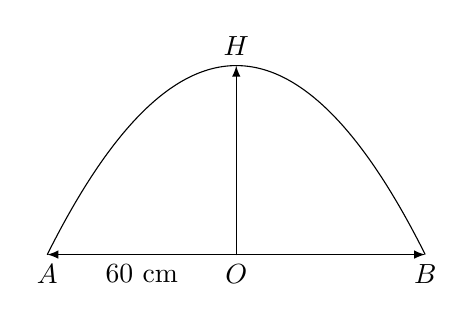
\begin{tikzpicture}[>=latex,smooth,line cap=round, line join=round, scale=0.8]
			\def\f(#1){-1/3*(#1)^2+3}
			\draw[->] (0,0)node[below]{$ O $}--(3,0) node[below]{$ B $};
			\draw[->] (-1.5,0) node[below]{$ 60 $ cm} (0,0)--(-3,0) node[below]{$ A $};
			\draw[->] (0,0)--(0,3) node[above] {$ H $};
			\draw[smooth,domain=-3:3,samples=200] plot (\x,{\f(\x)});
		\end{tikzpicture}
	}
	\loigiai{
		\immini{
			Chọn hệ trục tọa độ như hình vẽ. Đường viền chiếc gương là đường Parabol $ y=ax^2+bx+c\,(a\ne 0) $ có đỉnh $ H(0;30) $ và đi qua điểm $ B(30;0) $.\\
			Ta có: $ \begin{cases}
				c=30 \\ 
				-\dfrac{b}{2a}=0 \\ 
				900a+30b+c=0
			\end{cases}\Leftrightarrow\begin{cases}
				c=30 \\ 
				b=0 \\ 
				a=-\dfrac{1}{30}.
			\end{cases} $ \\
			Diện tích chiếc gương là diện tích hình phẳng giới hạn bởi Parabol $ y=-\dfrac{1}{30}x^2+30 $ và trục hoành.
		}
		{
			\begin{tikzpicture}[>=latex,smooth,line cap=round, line join=round, scale=0.8]
				\def\f(#1){-1/3*(#1)^2+3}
				\draw[->] (-4,0) -- (4,0) node[below] {$ x $};
				\draw[->] (0,-1) -- (0,4) node[right] {$ y $};
				\draw (0,0) node[below left]{$ O $} (3,0) node[below]{$ B $} (1.5,0) node[below]{$ 30 $ cm} (-3,0) node[below]{$ A $} (0,3) node[below right] {$ H $};
				\draw[smooth,domain=-3:3,samples=200] plot (\x,{\f(\x)});
			\end{tikzpicture}
		}
		\noindent Diện tích chiếc gương là
		$$S=\displaystyle\int_{-30}^{30}\left|-\dfrac{1}{30}x^2+30 \right|\mathrm{d}x=2\left| \displaystyle\int_0^{30}\left(-\dfrac{1}{30}x^2+30\right)\mathrm{d}x\right|=2\left|\left(-\dfrac{1}{90}x^3+30x\right)\bigg|_0^{30}\right|=1200\,(cm^2).$$
	}
\end{ex}
%%%=========HetCau_42=========%%%

%%%=========Cau_43=========%%%
\begin{ex}%[2H3B3-2]
	Trong không gian với hệ tọa độ $ Oxyz $, cho điểm $ A\left(1;-1;3\right) $ và hai đường thẳng $ d_1\colon\dfrac{x-4}{1}=\dfrac{y+2}{4}=\dfrac{z-1}{-2} $; $ d_2\colon\dfrac{x-2}{1}=\dfrac{y+1}{-1}=\dfrac{z-1}{1}$. PTĐT qua $ A $ vuông góc với $ d_1 $ và cắt $ d_2 $ là
	\choice
	{$ \dfrac{x-1}{4}=\dfrac{y+1}{1}=\dfrac{z-3}{4} $}
	{\True $ \dfrac{x-1}{2}=\dfrac{y+1}{-1}=\dfrac{z-3}{-1} $}
	{$ \dfrac{x-1}{-1}=\dfrac{y+1}{2}=\dfrac{z-3}{3} $}
	{$ \dfrac{x-1}{2}=\dfrac{y+1}{1}=\dfrac{z-3}{3} $}
	\loigiai{
		PTTS của đường thẳng $ d_1\colon\begin{cases}
			x=4+t \\ 
			y=-2+4t \\ 
			z=1-2t
		\end{cases} $ và $ d_2\colon\begin{cases}
			x=2+t \\ 
			y=-1-t \\ 
			z=1+t.
		\end{cases} $\\
		Phương trình mặt phẳng $ (P) $ qua $ A $ vuông góc với $ d_1 $ là $ x+4y-2z+9=0 $.\\
		Gọi $ H $ là giao điểm của $ (P) $ và đường thẳng $ d_2 $.
		$ H\in d_2\Rightarrow H(2+t;-1-t;1+t) $.\\
		$ H\in (P)\Rightarrow 2+t+4(-1-t)-2(1+t)+9=0\Leftrightarrow t=1. $ Vậy giao điểm $ H(3;-2;2) $.\\
		PTĐT qua $ A $ vuông góc với $ d_1 $ và cắt $ d_2 $ là PTĐT $ AH $ qua $ A(1;-1;3) $ và nhận $ \overrightarrow{AH}=(-2;1;1) $ làm véctơ chỉ phương.
	}
\end{ex}
%%%=========HetCau_43=========%%%

%%%=========Cau_44=========%%%
\begin{ex}%[2H1K3-2]
	Cho hình lăng trụ đứng $ ABC. A'B'C' $ có đáy $ ABC $ là tam giác vuông tại $ A $, $ \widehat{ACB}=30^\circ $, biết góc giữa $ B'C $ và mặt phẳng $ \left(ACC'A'\right) $ bằng $ \alpha $ thỏa mãn $ \sin\alpha=\dfrac{1}{2\sqrt{5}} $. Cho khoảng cách giữa hai đường thẳng $ A'B $ và $ CC' $ bằng $ a\sqrt{3} $. Tính thể tích $ V $ của khối lăng trụ $ ABC. A'B'C' $.
	\choice
	{\True $ V=2a^3\sqrt{3} $}
	{$ V=\dfrac{3a^3\sqrt{6}}{2} $}
	{$ V=a^3\sqrt{3} $}
	{$ V=a^3\sqrt{6} $}
	\loigiai{
		\immini{
			Ta có: $ CC'\parallel AA'\Rightarrow CC'\parallel (AA'B'B) $. Mà $ A'B\subset (AA'B'B),\, $ \\
			Nên
			$ \mathrm{d}(CC',A'B)=\mathrm{d}(CC',(AA'B'B))=C'A'=a\sqrt{3} $.\\
			Ta có $ AC=A'C'=a\sqrt{3} $, $ AB=A'B'=a $.\\
			Diện tích đáy là $ S_{ABC}=\dfrac{a^2\sqrt{3}}{2} $.\\
			Dễ thấy $ A'B'\perp (ACC'A') $. Góc giữa $ B'C $ và mặt phẳng $ (ACC'A') $ là $ \widehat{B'CA'}=\alpha $.\\
			$ \sin\alpha =\dfrac{A'B'}{B'C}=\dfrac{1}{2\sqrt{5}}\Leftrightarrow B'C=2a\sqrt{5} $.\\
			$ CC'=\sqrt{B'C^2}-B'C'^2=\sqrt{20a^2-4a^2}=4a $.\\
			Thể tích lăng trụ là $ V=B\cdot h $ với $ h=CC' $.\\
			Vậy $ V=\dfrac{a^2\sqrt{3}}{2}\cdot4a=2a^3\sqrt{3} $ .
		}
		{
			\begin{tikzpicture}[smooth,line cap=round, line join=round,font=\scriptsize,scale=0.8]
				\path
				(0,0) coordinate (A')
				($ (A')+(-45:3) $) coordinate (B')
				($ (A')+(0:5) $) coordinate (C')
				($ (A')+(90:5) $) coordinate (A)
				($ (A)+(B')-(A') $) coordinate (B)
				($ (A)+(C')-(A') $) coordinate (C);
				\draw (A)--(A')--(B')--(C')--(C)--(B')--(B)--(A)--(C)--(B)--(A');
				\draw[dashed] (C')--(A')--(C);
				\foreach \x/\g in {A/180,A'/180,B'/-90,B/180,C'/0,C/0}
				\fill [black] (\x) circle (1pt) + (\g:3mm) node {$ \x $};
			\end{tikzpicture}
		}
	}
\end{ex}
%%%=========HetCau_44=========%%%

%%%=========Cau_45=========%%%
\begin{ex}%[2D3K3-2]
	\immini{
		Cho Parabol $ (P)\colon y=x^2 $ và đường tròn $ (C) $ có tâm $ A(0;3) $, bán kính $ \sqrt{5} $ như hình vẽ. Diện tích phần được tô đậm giữa $ (C) $ và $ (P) $ gần nhất với số nào dưới đây?
		\choice
		{$ 1,77 $}
		{$ 3,44 $}
		{$ 1,51 $}
		{\True $ 3,54 $}
	}
	{
		\begin{tikzpicture}[>=latex,smooth,line cap=round, line join=round,scale=.8]
			\def\f(#1){(#1)^2}
			\pgfmathsetmacro{\a}{sqrt(5)}
			\pgfmathsetmacro\fb{\f(-2.2)}
			\draw[->] (-4,0) -- (4,0) node[below]{$ x $};
			\draw[->] (0,-1) -- (0,6) node[right] {$ y $};
			\fill[black] (0,0) node[below left]{$ O $} circle(2pt);
			\draw[name path=t] (0,3) circle (\a);
			\fill[black] (0,3) node[left]{$ A $} circle(2pt);
			\draw[smooth,domain=-2.2:2.2,name path=p] plot (\x,{\f(\x)});
			\path [name intersections={of=t and p, by={A,B,C,D}}];
			\draw[dashed,brown] let \p1=(A) in (\x1,\y1) let \p2=(B) in (\x2,\y2) let \p3=(C) in (\x3,\y3) let \p4=(D) in (\x4,\y4);
			\begin{scope}
				\clip (0,3) circle (\a);
				\fill[pattern=north east lines] (-\a,0)--plot[domain=-2.2:0] (\x,{\f(\x)})--(0,0)--cycle;
			\end{scope}
			\begin{scope}
				\clip (0,3) circle (\a);
				\fill[pattern=north east lines] plot[domain=0:2.2] (\x,{\f(\x)})--(\a,0)--(0,0)--cycle;
			\end{scope}
			\fill[pattern=north east lines] plot[domain=-1:1] (\x,{\f(\x)})--plot[domain=1:-1] (\x,{3-sqrt(5-(\x)^2)});
		\end{tikzpicture}
	}
	\loigiai{
		Phương trình $ (C)\colon x^2+(y-3)^2=5 $.\\
		Tọa độ giao điểm của $ (P) $ và $ (C) $ là nghiệm của hệ phương trình
		$$ \begin{aligned}
			\left\{\begin{aligned}
				& x^2+(y-3)^2=5 \\ 
				& y=x^2 \\ 
			\end{aligned}\right.&\Leftrightarrow \left\{\begin{aligned}
				& y+(y-3)^2=5 \\ 
				& y=x^2 \\ 
			\end{aligned}\right.\Leftrightarrow \left\{\begin{aligned}
				& \left[\begin{aligned}
					& y=1 \\ 
					& y=4 \\ 
				\end{aligned}\right. \\ 
				& y=x^2
			\end{aligned}\right.\\
			&\Leftrightarrow
			\left\{\begin{aligned}
				& x=1 \\ 
				& y=1 
			\end{aligned}\right. \text{ hay }\left\{\begin{aligned}
				& x=-1 \\ 
				& y=1 \\ 
			\end{aligned}\right. \text{ hay }\left\{\begin{aligned}
				& x=-2 \\ 
				& y=4 \\ 
			\end{aligned}\right. \text{ hay }\left\{\begin{aligned}
				& x=-2 \\ 
				& y=4 \\ 
			\end{aligned}\right.
		\end{aligned} $$
		Vậy tọa độ các giao điểm là $ (1;1) $, $ (-1;1) $, $ (-2;4) $, $ (2;4) $.\\
		Ta có: $ S=2\left(S_1+S_2\right) $.
		\begin{center}
			\begin{tikzpicture}[>=latex,smooth,line cap=round, line join=round]
				\def\f(#1){(#1)^2}
				\pgfmathsetmacro{\a}{sqrt(5)}
				\pgfmathsetmacro\fb{\f(-2.2)}
				\def\c{2}
				\def\d{1}
				\pgfmathsetmacro\fc{\f(\c)}
				\pgfmathsetmacro\fd{\f(\d)}
				\draw[->] (-4,0) -- (4,0) node[below]{$ x $};
				\draw[->] (0,-1) -- (0,6) node[right] {$ y $};
				\draw[name path=t] (0,3) circle (\a);
				\fill[black] (0,3) node[left]{$ A $} circle(2pt);
				\draw[smooth,domain=-2.2:2.2,name path=p] plot (\x,{\f(\x)});
				\begin{scope}
					\clip (0,3) circle (\a);
					\fill[pattern=north east lines] (-\a,0)--plot[domain=-2.2:0] (\x,{\f(\x)})--(0,0)--cycle;
				\end{scope}
				\begin{scope}
					\clip (0,3) circle (\a);
					\fill[pattern=north east lines] plot[domain=0:2.2] (\x,{\f(\x)})--(\a,0)--(0,0)--cycle;
				\end{scope}
				\fill[pattern=north east lines] plot[domain=-1:1] (\x,{\f(\x)})--plot[domain=1:-1] (\x,{3-sqrt(5-(\x)^2)});
				\draw[dashed] (-\c,0) node[below] {$ -\c $} -- (-\c,\fc)--(\c,\fc)--(\c,0) node[below] {$ \c $};
				\draw[dashed] (-\d,0) node[below] {$ -\d $} -- (-\d,\fd)--(\d,\fd)--(\d,0) node[below] {$ \d $} (0,4) node[above right] {$ 4 $} (0,0) node[below left] {$ O $};
				\draw[->] (1.2,0.5) node[right] {$ S1 $} -- (0.3,0.5);
				\draw[->] (2.2,1.5) node[right] {$ S2 $} -- (1.6,2);
			\end{tikzpicture}
		\end{center}		
		Tính $ S_1 $ : $ x^2+(y-3)^2=5\Rightarrow y=3-\sqrt{5-x^2}\Rightarrow S_1=\displaystyle\int_0^1\left[\left(3-\sqrt{5-x^2}\right)-x^2\right]\mathrm{d}x\approx 0,5075 $.\\
		Tính $ S_2 $: $\left\{\begin{aligned}
			& x^2+(y-3)^2=5\\
			& y=x^2
		\end{aligned}\right.\Rightarrow \left\{\begin{aligned}
			& x=\sqrt{5-(y-3)^2}\\
			& x=\sqrt{y}
		\end{aligned}\right.\Rightarrow \displaystyle\int_1^4 \left[\sqrt{5-(y-3)^2}-\sqrt{y}\right]\mathrm{d}y\approx1,26 $.\\
		Vậy $ S=2\left(S_1+S_2\right)\approx 3,54 $ 
	}
\end{ex}
%%%=========HetCau_45=========%%%

%%%=========Cau_46=========%%%
\begin{ex}%[2D3K2-2]
	Cho hàm số $ f(x) $ liên tục trên $ \mathbb{R} $ và thỏa $ \displaystyle\int_{-2}^2f\left(\sqrt{x^2+5}-x\right)\mathrm{d}x=1, $ 
	$ \displaystyle\int_1^5\dfrac{f(x)}{x^2}\mathrm{d}x=3. $ Tính $ \displaystyle\int_1^5f(x)\mathrm{d}x. $ 
	\choice
	{$ 0 $}
	{$ -15 $}
	{$ -2 $}
	{\True- $ 13 $}
	\loigiai{
		Đặt $ t=\sqrt{x^2+5}-x\Rightarrow x=\dfrac{5-t^2}{2t}\Rightarrow \mathrm{d}x=-\left(\dfrac{1}{2}+\dfrac{5}{2t^2}\right)\mathrm{d}t $.\\
		Ta có $ 1=\displaystyle\int_1^5f(t)\left(\dfrac{1}{2}+\dfrac{5}{2t^2}\right)\mathrm{d}t=\dfrac{1}{2}\displaystyle\int_1^5f(t)\mathrm{d}t+\dfrac{5}{2}\displaystyle\int_1^5\dfrac{f(t)}{t^2}\mathrm{d}t $.\\
		$ \Rightarrow \dfrac{1}{2}\displaystyle\int_1^5f(t)\mathrm{d}t=1-\dfrac{5}{2}\displaystyle\int_1^5\dfrac{f(t)}{t^2}\mathrm{d}t=1-\dfrac{5}{2}\cdot3=-\dfrac{13}{2} \Rightarrow \displaystyle\int_1^5f(t)\mathrm{d}t=-13 $.
	}
\end{ex}
%%%=========HetCau_46=========%%%

%%%=========Cau_47=========%%%
\begin{ex}%[2D4K2-2]
	Cho $ z,w \in\mathbb{C} $ thỏa $ |z+2|=\left|\overline{z}\right| $, $|z+i|=|z-i| $, $|w-2-3i|\le 2\sqrt{2} $, $ \left|\overline{w}-5+6i\right|\le 2\sqrt{2} $. Giá trị lớn nhất $ |z-w| $ bằng
	\choice
	{\True $ 5\sqrt{2} $}
	{$ 4\sqrt{2} $}
	{$ 3\sqrt{2} $}
	{$ 6\sqrt{2} $}
	\loigiai{
		Giả sử $ z=x+yi,\ (x,\,y\in \mathbb{R}) $. Gọi $ M(x;y) $ là điểm biểu diễn của $ z $ trên $ Oxy) $. Ta có
		\begin{enumerate}[$ \bullet $]
			\item $ |z+2|=\left|\overline{z}\right| \Leftrightarrow (x+2)^2+y^2=x^2+y^2 \Leftrightarrow x+1=0 $ ($ d_1 $).
			\item $ |z+i|=|z-i|\Leftrightarrow x^2+(y+1)^2=x^2+(y-1)^2\Leftrightarrow y=0 $ ($ d_2 $).
		\end{enumerate}
		Khi đó $ M=d_1\cap d_2 \Rightarrow M(-1;0) $.\\
		Giả sử $ w=a+bi $ ($ a,\, b\in \mathbb{R} $). Gọi $ N(a;b) $ là điểm biểu diễn của $ w $ trên $ (Oxy) $. Ta có
		\begin{enumerate}[$ \bullet $]
			\item $ |w-2-3i|\le 2\sqrt{2}\Leftrightarrow (a-2)^2+(b-3)^2\le 8 $ ($ C_1 $).
			\item $ \left| \overline{w}-5+6i\right| \le 2\sqrt{2}\Leftrightarrow (a-5)^2 + (b-6)^2\le 8 $ ($ C_2 $).
		\end{enumerate}
		Với $ (C_1) $ là hình tròn tâm $ I(2;3) $, bán kính $ R_1=2\sqrt{2} $, $ (C_2) $ là hình tròn tâm $ J(5;6) $, bán kính $ R_2=2\sqrt{2} $.
		Khi đó $ N $ thuộc miền chung của hai hình tròn $ (C_1) $ và $ (C_2) $ (hình vẽ).
		\begin{center}
			\begin{tikzpicture}[>=latex,smooth, line join=round, line cap=round,scale=0.6]
				\pgfmathsetmacro{\a}{2*sqrt(2)}
				\draw[->] (-3,0) -- (9,0) node[below]{$ x $};
				\draw[->] (0,-1) -- (0,10) node[right] {$ y $};
				\draw[name path=dcong] (2,3) circle (\a);
				\draw (5,6) circle (\a);
				\fill[black] (2,3)node[above] {$ I $} circle (2pt) (5,6) circle (2pt) node[above] {$ J $} (-1,0) circle (2pt) node[below]{$ M $} (4,5) circle (4pt) node[above] {$ N $};
				\draw (-1,0) -- (5,6);
			\end{tikzpicture}
		\end{center}
		Ta có $ |z-w| = MN $.\\
		Lại có $ \overrightarrow{MI} = (3;3) $, $ \overrightarrow{IJ}=(3;3)\Rightarrow \overrightarrow{MI}=\overrightarrow{IJ} $. Do đó ba điểm $ M $, $ I $, $ J $ thẳng hàng.\\
		Suy ra $ MN $ lớn nhất khi và chỉ khi $ N=MJ\cap (C_1)\Rightarrow MN_{\max} = MI+IN=3\sqrt{2}+2\sqrt{2}=5\sqrt{2} $.
	}
\end{ex}
%%%=========HetCau_47=========%%%

%%%=========Cau_48=========%%%
\begin{ex}%[2D2G5-2]
	Cho phương trình $ 3^x\left(3^{2x}+1\right)-\left(3^x+m+2\right)\sqrt{3^x+m+3}=2\sqrt{3^x+m+3} $, với $ m $ là tham số. Có bao nhiêu giá trị nguyên âm của $ m $ để phương trình có nghiệm thực?
	\choice
	{\True $3$}
	{$6$}
	{$4$}
	{$5$}
	\loigiai{
		Ta có
		$$\begin{aligned}
			&3^x\big(3^{2x}+1\big)-\big(3^x+m+2\big)\sqrt{3^x+m+3}=2\sqrt{3^x+m+3}\\
			\Leftrightarrow& 3^x\big(3^{2x}+1\big)=\big(3^x+m+2\big)\sqrt{3^x+m+3}+2\sqrt{3^x+m+3} \\
			\Leftrightarrow& 3^{3x}+3^x=\big(3^x+m+3\big)\sqrt{3^x+m+3}+\sqrt{3^x+m+3} \\
			\Leftrightarrow& 3^{3x}+3^x=\big(\sqrt{3^x+m+3}\big)^3+\sqrt{3^x+m+3}.
		\end{aligned}$$
		Xét hàm đặc trưng $ f(t)=t^3+t $ có $ f'(t)=3t^2+1>0,\forall t\in \mathbb{R} $.\\
		Vậy $ 3^{3x}+3^x=\big(\sqrt{3^x+m+3}\big)^3+\sqrt{3^x+m+3}\Leftrightarrow f\big(3^x\big)=f\big(\sqrt{3^x+m+3}\big) $ \\
		$ \Leftrightarrow 3^x=\sqrt{3^x+m+3}\Leftrightarrow 3^{2x}-3^x-3=m $. (*)\\
		Đặt $ u=3^x $, với điều kiện $ u>0 $ và đặt $ g(u)=u^2-u-3 $.\\
		Phương trình (*) $ \Leftrightarrow g(u)=m $.
		$ g'(u)=2u-1 $, $ g'(u)=0\Leftrightarrow u=\dfrac{1}{2} $, ta có bảng biến thiên của $ g(u) $:
		\begin{center}
			
\begin{tikzpicture}
				\tkzTabInit[nocadre,lgt=1.2,espcl=4,deltacl=0.7] {$ u $ /1, $ g'(u) $ /0.7, $ g(u) $ /2.5} {$ 0 $, $ \dfrac{1}{2} $, $ +\infty $}
				\tkzTabLine{,-,0,+,}
				\tkzTabVar{+/ $ -3 $,-/ $ -\dfrac{13}{4} $,+/ $ +\infty $}
			\end{tikzpicture}
		\end{center}
		Từ bảng biến thiên ta thấy phương trình đã cho có nghiệm thực khi và chỉ khi $ m>-\dfrac{13}{4} $.\\
		Vậy có tất cả 3 giá trị nguyên âm của $ m $ để phương trình có nghiệm thực là $ -3;\, -2;\, -1 $.
	}
\end{ex}
%%%=========HetCau_48=========%%%

%%%=========Cau_49=========%%%
\begin{ex}%[2H3K2-2]
	Trong không gian với hệ trục tọa độ $ Oxyz $, cho điểm $ A(2;1;3) $ và mặt phẳng $ (P)\colon x+my+(2m+1)z-m-2=0 $, $ m $ là tham số thực. Gọi $ H(a;b;c) $ là hình chiếu vuông góc của điểm $ A $ trên $ (P) $. Khi khoảng cách từ điểm $ A $ đến $ (P) $ lớn nhất, tính $ a+b $.
	\choice
	{$ 2 $}
	{$ \dfrac{1}{2} $}
	{\True $ \dfrac{3}{2} $}
	{$ 0 $}
	\loigiai{
		Ta có $ \mathrm{d}(A,(P))=\dfrac{\big| 2+m+3(2m+1)-m-2 \big|}{\sqrt{1^2+m^2+(2m+1)^2}}=\dfrac{3\big| 2m+1 \big|}{\sqrt{1+m^2+(2m+1)^2}} $.\\
		Vì $ 1+m^2\ge \dfrac{1}{5}(2m+1)^2$, $ \forall m\in \mathbb{R} $ nên $ \mathrm{d}(A,(P))\le \dfrac{3|2m+1|}{\sqrt{\dfrac{1}{5}(2m+1)^2+(2m+1)^2}}=\dfrac{\sqrt{30}}{2} $.\\
		Suy ra khoảng cách từ điểm $ A $ đến $ (P) $ là lớn nhất khi và chỉ khi $ m=2 $.\\
		Khi đó, $ (P)\colon x+2y+5z-4=0 $, $ AH\colon\left\{\begin{aligned}
			x=2+t \\
			y=1+2t \\
			z=3+5t.
		\end{aligned}\right. $ \\
		$ H=d\cap (P)\Rightarrow 2+t+2(1+2t)+5(3+5t)-4=0\Leftrightarrow t=-\dfrac{1}{2}\Rightarrow H\left(\dfrac{3}{2};0;\dfrac{1}{2}\right) $.\\
		Vậy $ a=\dfrac{3}{2},\,b=0\Rightarrow a+b=\dfrac{3}{2} $.
	}
\end{ex}
%%%=========HetCau_49=========%%%

%%%=========Cau_50=========%%%
\begin{ex}%[2D1G2-2]
	Cho hàm số $ y=f(x) $ có đạo hàm $ f'(x)=(x+1)^2(x+3)\left(x^2+2mx+5\right) $ với mọi $ x\in\mathbb{R} $. Có bao nhiêu giá trị nguyên âm của tham số $ m $ để hàm số $ g(x)=f\left(|x|\right) $ có đúng một điểm cực~trị.
	\choice
	{$ 3 $}
	{$ 5 $}
	{$ 4 $}
	{\True $ 2 $}
	\loigiai{
		$ f'(x)=(x+1)^2(x+3)\left(x^2+2mx+5\right)=0\Leftrightarrow \left[\begin{aligned}
			& x=-1 \\ 
			& x=-3 \\ 
			& x^2+2mx+5=0.\;\;(1) 
		\end{aligned}\right. $ \\
		Ta có: $ g(x)=\left\{\begin{aligned}
			& f(x)
			& \text{khi}
			& \;x\ge 0 \\ 
			& f(-x) 
			& \text{khi}
			& \;x<0.
		\end{aligned}\right. $ \\
		Hàm số $ y=g(x) $ có đúng 1 điểm cực trị
		$ \Leftrightarrow $ Hàm số $ y=f(x) $ không có điểm cực trị nào thuộc khoảng $ (0;+\infty) $.\\
		\textbf{\textit{Trường hợp 1:}} Phương trình $ (1) $ vô nghiệm hoặc có nghiệm kép
		\[\Leftrightarrow m^2-5\le 0\Leftrightarrow -\sqrt{5}\le m\le \sqrt{5}\;\;(*)\]
		\textbf{\textit{Trường hợp 2:}} Phương trình $ (1) $ có hai nghiệm $ x_1,x_2 $ phân biệt thoả mãn $ x_1<x_2\le 0 $ 
		$$ \Leftrightarrow \left\{\begin{aligned}
			& m^2-5>0 \\ 
			& -2m<0 \\ 
			& 5>0 \\ 
		\end{aligned}\right.\Leftrightarrow m>\sqrt{5}\;\;(**) $$.
		Từ (*) và (**) suy ra $ m\ge -\sqrt{5} $. Vì $ m $ là số nguyên âm nên $ m=\{-2;-1 \} $.
	}
\end{ex}
%%%=========HetCau_50=========%%%


\Closesolutionfile{ans}